\documentclass{beamer}

\usepackage[spanish,activeacute,es-tabla]{babel}
\usepackage[utf8]{inputenc} % mac utf8



\usepackage{graphicx}
\DeclareGraphicsExtensions{.png,.pdf,.jpg}

\usefonttheme{professionalfonts} % fuentes de LaTeX 
\usetheme{Boadilla}	% tema escogido en este ejemplo 



\setbeamertemplate{caption}[numbered]
\newtheorem{Teorema}{Teorema} 
\newtheorem{Definicion}{Definici\’on} 
\newtheorem{Prueba}{Prueba}

\theoremstyle{plain}

\newtheorem{teorema} [Teorema] {Teorema}
\newtheorem{definicion} [Definicion]{Definición} 
\newtheorem{lema} [theorem] {Lema}


\theoremstyle{example}
\newtheorem{Ejercicio}{Ejercicio} 
\newtheorem{ejercicio} [Ejercicio]{Ejercicio} 

\theoremstyle{example}
\newtheorem{Ejemplo}{Ejemplo} 
\newtheorem{ejemplo} [Ejemplo] {Ejemplo}

\setbeamertemplate{theorems}[numbered] 

% 3) Colores por defecto del style 'example' (fallback)
\setbeamercolor{block title example}{bg=green!40!black, fg=white}
\setbeamercolor{block body example}{bg=green!10, fg=black}

% 4) Colores por ENTORNO (locales) usando etoolbox
\usepackage{etoolbox}

% -- 'Ejemplo' en naranja
\AtBeginEnvironment{ejemplo}{%
  \setbeamercolor{block title example}{bg=orange!60!black, fg=white}%
  \setbeamercolor{block body example}{bg=orange!10, fg=black}%
}
% -- 'Ejercicio' en violeta
\AtBeginEnvironment{ejercicio}{%
  \setbeamercolor{block title example}{bg=violet!60!black, fg=white}%
  \setbeamercolor{block body example}{bg=violet!10, fg=black}%
}


\title[]{Tema 6. Códigos Lineales}

\author[José A Montenegro (jmmontes@uma.es)]{José A. Montenegro}
\institute{Dpto. Lenguajes y Ciencias de la Computación\\
ETSI Informática. Universidad de Málaga\\
jmmontes@uma.es
%\href{https://twitter.com//monteDocencia}{
%
\includegraphics[height=0.03\textheight]{twitter.jpg}}
}
\date{\today}



%###########################################################################
% FootLine
%###########################################################################

\setbeamertemplate{footline} {%
\leavevmode%
  \hbox{\begin{beamercolorbox}[wd=.5\paperwidth,ht=2.5ex,dp=1.125ex,leftskip=.3cm plus1fill,rightskip=.3cm]{author in head/foot}%
    \usebeamerfont{author in head/foot}\insertshortauthor 
  \end{beamercolorbox}%
  
  \begin{beamercolorbox}[wd=.5\paperwidth,ht=2.5ex,dp=1.125ex,leftskip=.3cm,rightskip=.3cm plus1fil]{title in head/foot}%
    Teoría de la Información y Codificación \hfill    \insertpagenumber /\insertdocumentendpage
  \end{beamercolorbox}}%
  \vskip0pt%
}%

%###########################################################################
% Document
%###########################################################################

\begin{document}

%\setbeamertemplate{headline}[title slide]
%\setbeamertemplate{footline}[title slide]


%###########################################################################
% Tíitulo
%###########################################################################
%\frame{\titlepage}
\begin{frame}

\includegraphics[height=0.15\textheight]{logoUma.jpg} \hspace*{3.5cm}

\includegraphics[height=0.17\textheight]{logoInf.jpg}   \hspace*{3.5cm}

\includegraphics[height=0.17\textheight]{logoLcc.jpg}  

\titlepage


\setbeamertemplate{footline}[body]
\setbeamertemplate{headline}[body]
\end{frame}

%###########################################################################
% Contenidos
%###########################################################################

\section[Resumen]{}
\frame{\tableofcontents}

%%%%%%%%%%%%%%%%%%%%%%%%%%%%%%%%
%%%%%%%%%%%%%%%%%%%%%%%%%%%%%%%%
%SECCION %%%%%%%%%%%%%%%%%%%%%%%%%%%%%%%
%%%%%%%%%%%%%%%%%%%%%%%%%%%%%%%%
%%%%%%%%%%%%%%%%%%%%%% 
\section{Introducción a códigos lineales}

\begin{frame}   \footnotesize
{
\setbeamercolor{block title}{bg=blue!60!black, fg=white}
\setbeamercolor{block body}{bg=blue!10, fg=black}
\begin{block}{Sección 1}
Introducción a códigos lineales
\end{block}
}
\end{frame} 

%%%%%%%%%%%%%%%%%%%%%%%%%%%%%%%%
\begin{frame} \frametitle{Introducción a códigos lineales} \footnotesize  

\begin{itemize} 
\item  Utilizaremos métodos algebraicos para construir códigos con el propósito de corregir los datos.
\item En alfabeto binario $\mathbb{B}$, los símbolos 0 y 1 pueden ser sumados y multiplicados acorde las siguientes reglas:

\begin{center}
$0+0=0, \; 0+1=1, \; 1+0=1, \;1+1=0$;
\end{center}
\begin{center}
$0\times 0=0, \; 0\times 1=0, \; 1\times 0=0, \; 1\times 1=1$.
\end{center}

\item  El conjunto $\mathbb{B}$, con estas operaciones es un \textbf{Cuerpo}, anotado como $\mathbb{F}_2$.

\item El conjunto $\mathbb{F}^n_2$ de palabras de longitud $n$ en $\mathbb{F}_2$ es un \textbf{espacio de vectores}. 

\item Las reglas para la suma de vectores y la multiplicación escalar son las siguientes:
\end{itemize} 

\begin{center}
$(x_1x_2 \ldots x_n)+(y_1y_2 \ldots y_n)=$ $(x_1+y_1$  $x_2+y_2 \ldots x_n+y_n); $
\end{center}

\begin{center}
$0\times (x_1x_2 \ldots x_n) = (00\ldots 0),	$
$1\times (x_1x_2 \ldots x_n) = (x_1x_2 \ldots x_n).$
\end{center}
\end{frame} 


%%%%%%%%%%%%%%%%%%%%%%%%%%%%%%%%
\begin{frame}  \small  

\begin{itemize} 
\item Un subconjunto C del espacio de vectores $\mathbb{F}^n_2$ es un \textbf{subespacio} si cualquier $x, y \in C$ cumple $x+y \in C$.
\end{itemize}

\begin{definicion}[Código Lineal]
Un código lineal (binario) es un subespacio C del espacio de vectores $\mathbb{F}^n_2$.
\end{definicion}

\begin{itemize} 

\item  El subconjunto $C = \{000,110,011\}$ de  $\mathbb{F}^3_2$ no es un código lineal, debido a que 110 + 011 = 101, el cual no está en C.


\item Por otro lado, el código repetición $R_n \subseteq \mathbb{F}^n_2$, contiene las dos palabras $000 \ldots 00$ y $111 \ldots 11$ es un código lineal para cualquier n, ya que $111 \ldots 11 + 111 \ldots 11 = 000 \ldots 00$. 


\end{itemize} \end{frame} 
%%%%%%%%%%%%%%%%%%%%%%%%%%%%%%%%
\begin{frame}  \footnotesize  
\begin{itemize}

 \item  Hemos establecido que la construcción de códigos requiere un compromiso entre \textbf{la tasa de información} $\rho$ y \textbf{la distancia mínima} $\delta$. 
 
\item Código lineal C es un subespacio de $\mathbb{F}^n_2$ tiene una \textbf{dimensión k}, definida como el tamaño del conjunto mínimo de expasión (bases). Es decir, un conjunto mínimo de vectores que permite generar todo el espacio por combinaciones lineales.

\item Cada elemento de C puede ser expresado de forma única como \textbf{una combinación lineal de la bases}, por lo que $|C| = 2^k$ para algún $k$ en el rango $0 \leq k \leq n$. 

\item Debido a que la tasa de información de C es: $\rho = \frac{log_2|C|}{n} = \frac{k}{n}$. Utilizamos $k$ en vez de $\rho$ y usualmente describiremos un \textbf{código lineal} por los parámetros \textcolor{red}{\textbf{$(n, k, \delta)$}}. 

\item Encontrar $\delta$ es tedioso, pero para un código lineal es más fácil.

\end{itemize}
\begin{definicion}[Peso]
El peso w(x) de una palabra $x \in \mathbb{F}_2^n$ es el número de 1s en x. 

Equivalentemente, w(x)=d(x,0), donde 0 denota la palabra de todos los ceros $000 \ldots 000$
\end{definicion}


\begin{lema}
Para un código lineal, la mínima distancia $\delta$ es igual al mínimo peso de una palabra codificada que no es $000 \ldots 000$.
\end{lema}

 \end{frame} 


%%%%%%%%%%%%%%%%%%%%%%%%%%%%%%%%
\begin{frame}  \small  
\begin{ejemplo}
Establezca los parámetros $(n, k, \delta)$ de los siguientes códigos lineales.

\begin{center}
$D_1 = \{000000,100000,010000,110000\},$
$D_2 = \{000000,111000,000111,111111\}.$
\end{center}
\end{ejemplo}

%\pause
\textit{\underline{Solución}}:\\
\vspace{0.3cm}
\begin{enumerate}
\item $D_1$ tiene palabra de longitud n=6 y ya que hay $4 = 2^2$ palabras codificadas, la dimensión es k=2 (y la tasa es $\rho=1/3$). 

\begin{itemize}
\item El peso de las palabras codificadas distintas de cero es 1,1,2 por lo que $\delta=1$.
\item Con este código, no es posible la corrección de errores. 
\end{itemize}

\item $D_2$ también tiene dimensión y tasa 1/3, pero la distancia mínima es $\delta = 3$, y es un código de corrección de errores de 1 bit.


\end{enumerate}


\end{frame} 
%%%%%%%%%%%%%%%%%%%%%%%%%%%%%%%%
\begin{frame}  \small  

\begin{itemize}
\item La construcción de los códigos lineales C con los valores de los parámetros $(n,k,\delta)$ está limitado por el límite de embalaje. 
\item Cuando $|C| = 2^k$, y $\delta  \geq 2r + 1$ (por lo que C es un código de error r) la condición es 

\end{itemize}



\[
 2^k \left( 1+ 
            \left( \begin{array}{c}
                  n \\
                  1       
           			\end{array}
    		\right) + 
    		\left( \begin{array}{c}
                  n  \\
                  2      
           			\end{array}
    		\right)+ \ldots + 
              \left( \begin{array}{c}
                  n \\
                  r      
           			\end{array}
    		\right)     		    		
    \right)    	\leq 2^{n}    		
\]


\end{frame} 

%%%%%%%%%%%%%%%%%%%%%%%%%%%%%%%%
\begin{frame}  \small  

\begin{ejemplo}

Establezca un límite superior para el número de palabras codificadas en un código lineal con longitud  de palabra 12, si necesitamos un código corrector error 2.\\
\end{ejemplo}

\textit{\underline{Solución}}:\\

\begin{itemize}
\item El límite de embalaje es $2^k(1 + 12 + 66) \leq 4096$, por lo que $2^k \leq 50$ aproximadamente. 

\item Ya que $k$ debe ser un entero el máximo posible de $2^k$ es $2^5=32$. 

\item (Aún no hemos determinado como construir tal código).

\end{itemize}

\end{frame} 



%%%%%%%%%%%%%%%%%%%%%%%%%%%%%%%%
%%%%%%%%%%%%%%%%%%%%%%%%%%%%%%%%
%\begin{frame}  \small \begin{ejercicio} \end{ejercicio} \pause \textit{\underline{Solución}}:\\ \end{frame} 
%%%%%%%%%%%%%%%%%%%%%%%%%%%%%%%%
%%%%%%%%%%%%%%%%%%%%%%%%%%%%%%%%
%EJERCICIO %%%%%%%%%%%%%%%%%%%%%%%%%%%%%%%
%%%%%%%%%%%%%%%%%%%%%%%%%%%%%%%%

%%%%%%%%%%%%%%%%%%%%%%%%%%%%%%%%
\begin{frame}  \small \begin{ejercicio} 
¿Cual de los siguientes subconjuntos de $\mathbb{F}^3_2$ es un código lineal? $C_1 = \{000, 110, 101, 011\}$, $C_2 = \{000, 100, 010, 001\}$.

\end{ejercicio} %\pause 
\textit{\underline{Solución}}:\\ 
\vspace{0.3cm}
\begin{description}
\item[$C_1$] 110+101= 011, 110+011= 101, 101+011= 110.
\item[$C_2$] 100+010= 110 No pertenece a $C_2$.
\end{description}

\end{frame} 

%%%%%%%%%%%%%%%%%%%%%%%%%%%%%%%%
%%%%%%%%%%%%%%%%%%%%%%%%%%%%%%%%

\begin{frame}  \small \begin{ejercicio} 

Supongamos que queremos enviar uno entre 128 mensajes diferentes, y cada mensaje esta representado por una palabra codificada de longitud 10.\\
\vspace{0.1cm}
¿Es posible construir un código linear corrector-1 que satisface estas condiciones?

\end{ejercicio} %\pause 
\textit{\underline{Solución}}:\\ 
\vspace{0.3cm}
n= 10, k= 7\\

\vspace{0.1cm}

Según el límite de embalaje tenemos:\\
\vspace{0.1cm}
$2^k (1+n) \leq 2^n$, $128 (1+10) \leq 1024$, $1408 \leq 1024$\\
\vspace{0.1cm}
No se cumple.

\end{frame} 

%%%%%%%%%%%%%%%%%%%%%%%%%%%%%%%%

%%%%%%%%%%%%%%%%%%%%%%%%%%%%%%%%
%%%%%%%%%%%%%%%%%%%%%%%%%%%%%%%%
\begin{frame}  \small \begin{ejercicio} 

Es necesario asignar a cada estudiante un número identificativo mediante una palabra binaria.\\

(a) Si hay 53 estudiantes, encuentra menor dimensión posible de un código lineal para este propósito.\\ 

(b) Si el código debe permitir la corrección de 1 error, encontrar la menor longitud posible de las palabras codificadas.


\end{ejercicio} %\pause 
\textit{\underline{Solución}}:\\ 
\vspace{0.3cm}

a) $53. 2^6$

b) $2^6 (1+n) \leq 2^n; 1+n \leq 2^{(n-6)};   (n=10); $
\end{frame} 
%%%%%%%%%%%%%%%%%%%%%%%%%%%%%%%%



%%%%%%%%%%%%%%%%%%%%%%%%%%%%%%%%
%%%%%%%%%%%%%%%%%%%%%%%%%%%%%%%%
\begin{frame}  \small \begin{ejercicio} 

Supongase que necesitamos construir un código lineal con n=12 y $\delta =3$. Encuentra un límite superior para la tasa de información del código mencionado.

\end{ejercicio} %\pause 
\textit{\underline{Solución}}:\\ 
\vspace{0.3cm}

$2^k (1+12) \leq 2^{12};  2^k  \leq 2^{12} /13;  2^k  \leq  315; k=8$

$\rho = k / n; \rho = 8 /12, \rho = 2/3$

\end{frame} 
%%%%%%%%%%%%%%%%%%%%%%%%%%%%%%%%




%8.5. Given words x,y ∈ F2n let x ∗ y denote the word that has 1 in any position if and only if both x and y have 1 in that position. Prove that w(x + y) = w(x) + w(y) − 2w(x ∗ y). Deduce that the set of all words with even weight in F2n is a linear code.


%%%%%%%%%%%%%%%%%%%%%%%%%%%%%%%%
%%%%%%%%%%%%%%%%%%%%%%%%%%%%%%%%
\begin{frame}  \small \begin{ejercicio} 

Sea $B(n,\delta)$ que denota la máxima dimensión de un código lineal en $\mathbb{F}_2^n$ con mínima distancia $\delta$. Haciendo uso del límite de embalaje mostrar que $B(6,3) \leq 3$,	$B(7,3) \leq 4$,	$B(8,3) \leq 4$.

\end{ejercicio} %\pause 
\textit{\underline{Solución}}:\\ 
\vspace{0.3cm}

$2^k (1+6) \leq 2^6; 2^k \leq 9,14. k =3$

$2^k (1+7) \leq 2^7; 2^k \leq 16. k=4$

$2^k (1+8) \leq 2^8; 2^k \leq 28.4. k=4$

\end{frame} 

%%%%%%%%%%%%%%%%%%%%%%%%%%%%%%%%





%%%%%%%%%%%%%%%%%%%%%%%%%%%%%%%%
%SECCION %%%%%%%%%%%%%%%%%%%%%%%%%%%%%%%
%%%%%%%%%%%%%%%%%%%%%%%%%%%%%%%%
\section{Construcción de códigos lineales utilizando matrices}


\begin{frame}   \footnotesize
{
\setbeamercolor{block title}{bg=blue!60!black, fg=white}
\setbeamercolor{block body}{bg=blue!10, fg=black}
\begin{block}{Sección 2}
Construcción de códigos lineales utilizando matrices
\end{block}
}
\end{frame} 
%%%%%%%%%%%%%%%%%%%%%%%%%%%%%%%%
\begin{frame}  \frametitle{Construcción de códigos lineales utilizando matrices}\small  
\begin{itemize} 

\item Cuando vimos el problema de transmitir información según una \textbf{tasa} establecida ($\rho$), mientras reducimos la \textbf{probabilidad de confusión} ($M(C_n,p)$). La idea principal es dividir el \textbf{flujo original de bits} en \textcolor{red}{bloques de tamaño k} y asignar una \textcolor{red}{palabra codificada de longitud n} a cada uno de los $2^k$ posibles bloques. 

\item Es decir,  una \textbf{función de codificación} $\mathbb{F}_2^k \rightarrow \mathbb{F}_2^n$. 

\item Dado que $\mathbb{F}_2^k$ y $\mathbb{F}_2^n$ son espacio de vectores,  un candidato para tal función es una \textbf{transformación lineal}, definida por una \textbf{matriz}.

\item \textcolor{red}{\textbf{E}} es una $n \times k$ matriz en $\mathbb{F}_2$ e $y$ un vector en  $\mathbb{F}_2^k$, entonces la palabra x definida por $x'=Ey'$ está en $\mathbb{F}_2^n$. 

\item La \textcolor{red}{\textbf{matriz  E}} define \textbf{una función de codificación} $\mathbb{F}_2^k \rightarrow \mathbb{F}_2^n$.

\end{itemize} \end{frame} 
%%%%%%%%%%%%%%%%%%%%%%%%%%%%%%%%

\begin{frame}  \footnotesize

\begin{ejemplo} \label{ej:bloqueCodigo2}

En el ejemplo del tema anterior establecimos una regla que asignaba a cada bloque $y_1y_2y_3$ de tamaño 3 una palabra codificada $x_1x_2x_3x_4x_5x_6$ de tamaño 6. Expresa esta regla en forma de matriz.

\begin{center}
$x_1 = y_1$\\
$x_2 = y_2$\\
$x_3 = y_3$\\
$x_4 =0$ si $y_1 =y_2$, si no $x_4 =1$\\
$x_5 =0$ si $y_2 =y_3$, si no $x_5 =1$\\
$x_6 =0$ si $y_1 =y_3$, si no $x_6 =1$\\
\end{center}

\end{ejemplo}
\end{frame} 

%%%%%%%%%%%%%%%%%%%%%%%%%%%%%%%%
\begin{frame}  \footnotesize

\textit{\underline{Solución}}:\\
\vspace{0.1cm}
La regla para $x_4$ es $x_4 =0$ si $y_1 =y_2$, si no $x_4 =1$. Utilizando la estructura algebraica del cuerpo $\mathbb{F}_2$ podemos expresarlos mediante una ecuación lineal $x_4= y_1 + y_2$. De las misma forma tenemos $x_5= y_2 + y_3$ y  $x_6= y_1 + y_3$. Todas las ecuaciones pueden ser escritas mediante una simple ecuación de matrices.


\[
            \left( \begin{array}{c}
                  x_1 \\
                  x_2  \\   
                  x_3 \\
                  x_4  \\
                  x_5 \\
                  x_6   
           			\end{array}
    		\right) = 
            \left( \begin{array}{c}
                  y_1 \\
                  y_2  \\   
                  y_3 \\
                  y_1 + y_2  \\
                  y_2 + y_3 \\
                  y_1 + y_3  
           			\end{array}
    		\right) = E
    		\left( \begin{array}{c}
                  y_1  \\                        
                  y_2  \\
                  y_3
           			\end{array}
    		\right) 		    		
\]

donde $E$ es la matriz 6 x 3 siguiente:

\[
   E=      \left( \begin{array}{ccc}
                  \textcolor{red}{1} & 0 & 0 \\
                  0 & \textcolor{red}{1} & 0  \\   
                  0 & 0 & \textcolor{red}{1} \\
                  1 & 1 & 0   \\
                  0 & 1 & 1  \\
                  1 & 0 & 1   
           			\end{array}
    		\right) 	    		
\]

El código resultante $C\subseteq \mathbb{F}_2^6$ tiene los parámetros n = 6, k = 3, and $\delta = 3$, y por tanto es un código corrector de error 1 con una tasa 1/2.

\end{frame} 

%%%%%%%%%%%%%%%%%%%%%%%%%%%%%%%%
\begin{frame}  \small  
\begin{itemize} 

\item  En general, dado cualquier matriz $E$ (n x k) sobre $\mathbb{F}_2$, sea \textcolor{red}{\textbf{C el conjunto}} 

\begin{center}
 \{$x \in \mathbb{F}_2^n$ $|$ x' =E y' \; \; para algún $y \in \mathbb{F}_2^k$\}.
\end{center}

\begin{itemize} 
\item Si $x$ y $w$ pertenecen a  $C$, tenemos que $x'=Ey'$ y $w' =Ez'$, entonces (x+w)' =E (y+z)', por lo que x + w también están en C, por tanto C es\textbf{ un código lineal}.
\end{itemize} 

\item Esencialmente, ahora tenemos la respuesta al \textbf{problema de codificar un flujo de bits}. 


\begin{itemize} 

\item El flujo es \textbf{dividido en bloques} $y$ de longitud $k$, y la \textbf{palabra codificada} para $y$ es $x$, donde $x'=Ey'$, para una matriz $E$ apropiada. 
\vspace{0.2cm}
\item Debemos intentar asegurar que el código resultante tiene buenas propiedades de corrección de errores, y que existe un método para implementar la \textbf{regla MD}, que veremos a continuación.
\end{itemize} 

\end{itemize} 


\end{frame} 

%%%%%%%%%%%%%%%%%%%%%%%%%%%%%%%%
%%%%%%%%%%%%%%%%%%%%%%%%%%%%%%%%
%\begin{frame}  \small \begin{ejercicio} \end{ejercicio} \pause \textit{\underline{Solución}}:\\ \end{frame} 
%%%%%%%%%%%%%%%%%%%%%%%%%%%%%%%%
%%%%%%%%%%%%%%%%%%%%%%%%%%%%%%%%
%EJERCICIO %%%%%%%%%%%%%%%%%%%%%%%%%%%%%%%
%%%%%%%%%%%%%%%%%%%%%%%%%%%%%%%%

%%%%%%%%%%%%%%%%%%%%%%%%%%%%%%%%
\begin{frame}  \small \begin{ejercicio} 
Supongamos que codificamos un bloque de bits $y_1 y_2 \ldots y_k$ estableciendo $x_i =y_i$ para $ i= 1,2,\ldots k$ y definimos el bit de verificación de paridad  $x_{k+1}$ como sigue: 

\vspace{0.2cm}
$x_{k+1} =0$ si hay un número par de yi's=1, $x_{k+1} =1$ si el número de yi's=1 son impar. 

\vspace{0.2cm}
Escribir la matriz E tal que x' = E y'.

\end{ejercicio} %\pause 
\textit{\underline{Solución}}:\\ 
\vspace{0.3cm}
La matriz sería la identidad para que los $x_1x_2 \ldots y_k$ y para $x_{k+1}$ sería toda la fila a 1.

Para el caso de k=3 sería:

\[
   E=      \left( \begin{array}{ccc}
                  1 & 0 & 0 \\
                  0 & 1 & 0  \\   
                  0 & 0 & 1 \\
                  1 & 1 & 1  
           			\end{array}
    		\right) 	    		
\]

\end{frame} 


%%%%%%%%%%%%%%%%%%%%%%%%%%%%%%%%
\begin{frame}  \small \begin{ejercicio} 
Mostrar que en el código definido en el ejercicio anterior cada palabra tiene un peso par.
\end{ejercicio} %\pause 
\textit{\underline{Solución}}:\\ 
\vspace{0.3cm}

Tenemos solamente dos casos.

a) La palabra tiene un peso par de 1 se añade un 0 en el código de control, con lo cual la palabra será par.\\
b) La palabra tiene un peso impar con lo cual se añade un 1 como código de control, y la palabra vuelve a ser par.

\end{frame} 

%%%%%%%%%%%%%%%%%%%%%%%%%%%%%%%%

%%%%%%%%%%%%%%%%%%%%%%%%%%%%%%%%
\begin{frame}  \small \begin{ejercicio} 

Establece la tasa de información $\rho$ y la mínima distancia $\delta$ para el código de verificación de paridad.

\end{ejercicio} %\pause 
\textit{\underline{Solución}}:\\ 
\vspace{0.3cm}
$\rho = \frac{k}{k+1}$\\

\vspace{0.4cm}
$\delta = 2$.  Mínimo par por el peso son 2.
\end{frame} 
%%%%%%%%%%%%%%%%%%%%%%%%%%%%%%%%






%%%%%%%%%%%%%%%%%%%%%%%%%%%%%%%%
%%%%%%%%%%%%%%%%%%%%%%%%%%%%%%%%
%%%%%%%%%%%%%%%%%%%%%%%%%%%%%%%%
%SECCION %%%%%%%%%%%%%%%%%%%%%%%%%%%%%%%
%%%%%%%%%%%%%%%%%%%%%%%%%%%%%%%%
\section{La matriz de verificación de un código lineal}


\begin{frame}   \footnotesize
{
\setbeamercolor{block title}{bg=blue!60!black, fg=white}
\setbeamercolor{block body}{bg=blue!10, fg=black}
\begin{block}{Sección 3}
La matriz de verificación de un código lineal
\end{block}
}
\end{frame} 
%%%%%%%%%%%%%%%%%%%%%%%%%%%%%%%%
\begin{frame} \frametitle{La matriz de verificación de un código lineal}\footnotesize  
\begin{itemize} 

\item Para codificar un flujo de bits \textbf{divido en bloques de longitud }$k$ y aplicando una \textbf{matriz} $E$ $(n \times k)$ para cada \textbf{bloque y}. 

\item En el ejemplo \ref{ej:bloqueCodigo2} la transformación $x' =E y'$ estaba definida por las siguientes ecuaciones lineales:

\begin{center}
$x_1 =y_1$,	 $x_2 =y_2$,	$x_3 =y_3$,\\
$x_4 =y_1 +y_2$,	$x_5 =y_2 +y_3$,	$x_6 =y_1 +y_3$.
\end{center}

\item Las variables \textcolor{red}{$y_1, y_2, y_3$ pueden ser eliminadas} de la ecuación, obteniendo

\begin{center}
$x_1 +x_2 +x_4 =0$,	$x_2 +x_3 +x_5=0$,	$x_1 +x_3 +x_6 =0$.
\end{center}

\tiny{
\begin{center}
Nota: -1 = 1 en el cuerpo $\mathbb{F}_2$. 
\end{center}
}

\footnotesize
\item Estas ecuaciones pueden ser reescritas de la forma de una ecuación de matrices $Hx' = 0'$, donde

\[
   H=      \left( \begin{array}{cccccc}
                  1 & 1 & 0 & 1 & 0 & 0\\
                  0 & 1 & 1 & 0 & 1 & 0  \\   
                  1 & 0 & 1 & 0 & 0 & 1  
           			\end{array}
    		\right) 	    		
\]

\item Una forma alternativa de definir el código, como  el conjunto de x tal que $Hx' = 0'$, que es un subespacio de $\mathbb{F}_2^n$ y por tanto un \textbf{código lineal}. 

\end{itemize} \end{frame} 

%%%%%%%%%%%%%%%%%%%%%%%%%%%%%%%%
\begin{frame}  \small  
\begin{lema}

Sea $E$ una matriz n x k sobre $\mathbb{F}_2$, de la forma

\[
  		\left( \begin{array}{c}
                  I \\
                  A   
           			\end{array}
    		\right) 	    		
\]

donde $I$ es la \textcolor{red}{\textbf{matriz identidad}} con tamaño k, y $A$ es cualquier matriz $(n - k) \times k$.\\
\vspace{0.2cm}
Entonces el código \{$x \in \mathbb{F}_2^n$ $|$ x' = \;E \;y' \; para algún $y \in \mathbb{F}_2^k$\} \textbf{puede ser definido como}  \{$x \in \mathbb{F}_2^n$ $|$ H x' =0'\} donde $H$ es la $(n - k) \times n$ matriz (A I).  
\vspace{0.2cm}

($I$ es la matriz identidad con tamaño $n - k$.)\\

\end{lema}


\end{frame} 

%%%%%%%%%%%%%%%%%%%%%%%%%%%%%%%%
\begin{frame}  \small  

\begin{definicion}[Matriz Verificación]
Una matriz H en $\mathbb{F}_2$ con m filas y n columnas es la \textcolor{red}{\textbf{matriz de verificación}} para el código lineal

\begin{center}
$C = \{x \in F_2^n |\; Hx' = 0'\}.$
\end{center}
\end{definicion}

En la definición $H$ puede ser cualquier matriz m x n sobre $\mathbb{F}_2$.\\  
\vspace{0.2cm}
H tiene la forma estándar $(A I)$, donde $A$ tiene n-m columnas y $I$ tiene m columnas.\\ 
\vspace{0.2cm}
Entonces el código correspondiente tiene dimensiones k = n - m. 

\[
   H=  (A I) =     \left( \begin{array}{ccccccccc}
                  a_{11} & a_{12} & \ldots & a_{1k} & & 1 & 0 & \ldots & 0\\
                  a_{21} & a_{22} & \ldots & a_{2k} & & 0 & 1 & \ldots & 0\\
                  . & . & \ldots & . & & . & . & \ldots & .\\
                  . & . & \ldots & . & & . & . & \ldots & .\\
                  a_{m1} & a_{m2} & \ldots & a_{mk} & & 0 & 0 & \ldots & 1
           			\end{array}
    		\right) 	    		
\]

 \end{frame} 


%%%%%%%%%%%%%%%%%%%%%%%%%%%%%%%%
\begin{frame}  \footnotesize  

Por tanto las ecuaciones $Hx' = 0'$ son

\begin{center}
$a_{11} x_1+ a_{12} x_2 + \ldots + a_{1k} x_k + x_{k+1} =0$\\
$a_{21} x_1+ a_{22} x_2 + \ldots + a_{2k} x_k + x_{k+2} =0$\\
$\ldots$ $\ldots$\\
$a_{m1} x_1+ a_{m2} x_2 + \ldots + a_{mk} x_k + x_{n} =0$\\
\end{center}

Estas ecuaciones pueden ser reordenadas de forma que los valores  $x_{k+1},x_{k+2}, \ldots x_n$ son definidos en términos de los valores $x_1,x_2,\ldots,x_k$: 

\begin{center}
$ x_{k+1} = a_{11} x_1+ a_{12} x_2 + \ldots + a_{1k} x_k$\\
$ x_{k+2} = a_{21} x_1+ a_{22} x_2 + \ldots + a_{2k} x_k$\\
$\ldots$ $\ldots$\\
$x_{k+2} = a_{m1} x_1+ a_{m2} x_2 + \ldots + a_{mk} x_k$\\
\end{center}

En una palabra codificada $x = x_1x_2 \ldots x_n$, estableceremos que

\begin{center}
$x_1,x_2,\ldots, x_k$ son \textbf{los bits de los mensajes}\\
$x_{k+1},x_{k+2},\ldots, x_n$ son \textbf{los bits de verificación}.
\end{center}

Si asignamos valores a los bits de mensajes, podremos determinar los valores de los bits de verificación con las ecuaciones establecidas. 

\end{frame} 
%%%%%%%%%%%%%%%%%%%%%%%%%%%%%%%%
%\begin{frame}  \small  
%\begin{itemize} 

%\item En una palabra codificada $x = x_1x_2 \ldots x_n$, estableceremos que

%\begin{center}
%$x_1,x_2,\ldots, x_k$ son \textbf{los bits de los mensajes}\\
%$x_{k+1},x_{k+2},\ldots, x_n$ son \textbf{los bits de verificación}.
%\end{center}

%\item Si los bits de mensajes tienen asignados valores arbitrarios, los valores de los bits de verificación son determinados por las ecuaciones anteriormente explicados. 

%\item Ya que tenemos $2^k$ posibles valores de mensajes, la dimensión del código es $k$.

%\end{itemize} \end{frame} 


%%%%%%%%%%%%%%%%%%%%%%%%%%%%%%%%
\begin{frame}  \small  

\begin{ejemplo}\label{ej:CodeMatrizV}

Establezca  una lista de las palabras codificadas definidas por la matriz de verificación

\[
   H=      \left( \begin{array}{cccc}
                  1 & 0 & 1 & 0\\
                  1 & 1 & 0 & 1 	  
           			\end{array}
    		\right) 	    		
\]

¿Cuales son los parámetros de este código?\\
\end{ejemplo}
\end{frame} 


%%%%%%%%%%%%%%%%%%%%%%%%%%%%%%%%
\begin{frame}  \footnotesize 

\textit{\underline{Solución}}:\\

Si $x = x_1x_2x_3x_4$ entonces la condición $Hx' = 0'$ tenemos que  

\begin{center}
$x_1 +x_3 =0$,	$x_1 +x_2 +x_4 =0.$
\end{center}

Podemos reescribir las ecuaciones de forma que $x_3$ y $x_4$ son dados en términos de $x_1$ y $x_2$:

\begin{center}
$x_3 = x_1$,	$x_4 = x_1 + x_2$.
\end{center}

Las \textbf{palabras codificadas (c)}  pueden ser encontradas dando todos los posibles valores a $x_1$, $x_2$ y utilizando las ecuaciones para calcular $x_3$ y $x_4$.

\[
        \left( \begin{array}{ccccc}
                  x_1 & x_2 & x_3 & x_4 & peso\\
                      0 &   0   &   0  &    0 &	0\\ 
					  0 &   1   &   0  &    1 &	2\\ 
					  1 &   0   &   1  &    1 &	3\\ 
					  1 &   1   &   1  &    0 &	3
           			\end{array}
    		\right) 	    		
\]

El código tiene parámetros n=4, k=2, y la mínima distancia es igual al mínimo peso que no es cero, el cual es $\delta =2$.


\end{frame} 

%%%%%%%%%%%%%%%%%%%%%%%%%%%%%%%%
%%%%%%%%%%%%%%%%%%%%%%%%%%%%%%%%
%\begin{frame}  \small \begin{ejercicio} \end{ejercicio} \pause \textit{\underline{Solución}}:\\ \end{frame} 
%%%%%%%%%%%%%%%%%%%%%%%%%%%%%%%%
%%%%%%%%%%%%%%%%%%%%%%%%%%%%%%%%
%EJERCICIO %%%%%%%%%%%%%%%%%%%%%%%%%%%%%%%
%%%%%%%%%%%%%%%%%%%%%%%%%%%%%%%%

%%%%%%%%%%%%%%%%%%%%%%%%%%%%%%%%
\begin{frame}  \small \begin{ejercicio} 

Establece una lista de palabras codificadas definidas por la matriz de verificación

\[
H=  \left( \begin{array}{ccccc}
                  1 & 0 & 1 & 0 & 0\\
                  1 & 1 & 0 & 1 & 0\\
                  0 & 1 & 0 & 0 & 1
           			\end{array}
    		\right) 	    		
\]

¿Cuales son los parámetros de este código?

\end{ejercicio} 


 \end{frame} 
%%%%%%%%%%%%%%%%%%%%%%%%%%%%%%%%

%%%%%%%%%%%%%%%%%%%%%%%%%%%%%%%%
\begin{frame}  \footnotesize

 \textit{\underline{Solución}}:\\
Si $x = x_1x_2x_3x_4$ entonces la condición $Hx' = 0'$ tenemos que  

\begin{center}
$x_1 +x_3 =0$,	$x_1 +x_2 +x_4 =0$,	$x_2 +x_5 =0.$
\end{center}

Podemos reescribir las ecuaciones de forma que $x_3$ $x_4$ y $x_5$ son dados en términos de $x_1$ y $x_2$:

\begin{center}
$x_3 = x_1$,	$x_4 = x_1 + x_2$, $x_5 = x_2$
\end{center}

\[
        \left( \begin{array}{cccccc}
                  x_1 & x_2 & x_3 & x_4 & x_5 & peso\\
                      0 &   0   &   0  &    0 &   0  &0\\  
					  0 &   1   &   0  &    1 &   1  &3\\ 
					  1 &   0   &   1  &    1 &   0  &3\\ 
					  1 &   1   &   1  &    0 &   1  &4
           			\end{array}
    		\right) 	    		
\]

El \textbf{código} tiene parámetros n=5, k=2, y la mínima distancia es igual al mínimo peso que no es cero, el cual es $\delta =3$.


 \end{frame} 
%%%%%%%%%%%%%%%%%%%%%%%%%%%%%%%%


%8.11. Write down a check matrix for the parity check code described in Exercise 8.7.


%%%%%%%%%%%%%%%%%%%%%%%%%%%%%%%%
%%%%%%%%%%%%%%%%%%%%%%%%%%%%%%%%
%\begin{frame}  \small \begin{ejercicio} 
%El código $C_1 =\{00,01,10,11\}$ pude ser usado para representar 4 mensajes $\{a,b,c,d\}$. El código $C_r$ es obtenido mediante repetición de cada palabra en $C_1$ r veces: por ejemplo, en $C_3$ el mensaje b es representado por 010101. Muestra que $C_r$ es un código lineal y establece sus parámetros $(n,k,\delta)$ y la matriz de verificación asociada.

%\end{ejercicio} %\pause 
%\textit{\underline{Solución}}:\\ 
%\vspace{0.3cm}
%Ya que $C_1$ es lineal por extensión podemos determinar que  $C_r$ es lineal.

%Los parámetros son n = 2r,k=2,$\delta=r$. 

%La matriz de verificación representa estas ecuaciones $x_1=x_3 = x_5=\ldots$ y  $x_2=x_4 = x_6=\ldots$


%º\end{frame} 
%%%%%%%%%%%%%%%%%%%%%%%%%%%%%%%%



%%%%%%%%%%%%%%%%%%%%%%%%%%%%%%%%
%%%%%%%%%%%%%%%%%%%%%%%%%%%%%%%%
%SECCION %%%%%%%%%%%%%%%%%%%%%%%%%%%%%%%
%%%%%%%%%%%%%%%%%%%%%%%%%%%%%%%%
\section{Construyendo códigos correctores 1 bit}

\begin{frame}   \footnotesize
{
\setbeamercolor{block title}{bg=blue!60!black, fg=white}
\setbeamercolor{block body}{bg=blue!10, fg=black}
\begin{block}{Sección 4}
Construyendo códigos correctores 1 bit
\end{block}
}
\end{frame} 
%%%%%%%%%%%%%%%%%%%%%%%%%%%%%%%%
\begin{frame}  \frametitle{Construyendo códigos correctores 1 bit} \small  
El siguiente teorema describe una forma muy fácil para construir una matriz de verificación para un código corrector 1 bit.

\begin{teorema}\label{teo:Hdef}

El Código C definido por una \textbf{matriz de verificación} $H$ es un \textbf{código corrector 1} cumpliendo que 

\begin{enumerate}
\item No existe una columna en $H$ con todos los elementos 0s.
\item No tenemos dos columnas de H idénticas.
\end{enumerate}

\end{teorema}

\end{frame} 


%%%%%%%%%%%%%%%%%%%%%%%%%%%%%%%%
\begin{frame}  \footnotesize  

\begin{ejemplo}

En un ejemplo anterior mostramos que el menor valor posible de n y k para un código corrector 1 con tasa de información 0.8 son n=25, k=20.\\
\vspace{0.2cm}
¿Como podemos construir el código utilizando una matriz de verificación?\\

\end{ejemplo}

\textit{\underline{Solución}}:\\

\begin{itemize}
\item $H$ es una matriz m x n con m=n-k = 5 filas.
\item Acorde con el teorema \ref{teo:Hdef}, las n= 25 columnas deben ser distintas, y ninguna columna puede ser cero. 

\item Concretamente hay $2^5 -1=31$ posibles columnas y cualquiera  25 de esas columnas puedan ser elegidas.

\item Si $H$ esta en forma estándar las últimas cinco columnas serán 5 palabras de peso 1, 
\item y las primeras 20 columnas pueden ser cualquiera palabra que no sea cero y distintas a las 5 últimas columnas.
\end{itemize}

\end{frame} 

%%%%%%%%%%%%%%%%%%%%%%%%%%%%%%%%
\begin{frame}  \footnotesize  

\begin{teorema}\label{ithBIT}

Sea $C \subseteq \mathbb{F}_2^n$ un código lineal definido por una\textbf{ matriz de verificación} $H$. \\
\vspace{0.1cm}
Suponemos que \textbf{un error en un bit} sucede en la transmisión de una palabra codificada (palabra recibida es z). \\
\vspace{0.1cm}
El \textbf{error} ocurre en el $i^{th}$ bit de $z$, donde $i$ es determinado por el hecho que $Hz'$ es igual a la $i^{th}$ columna de $H$. 
\end{teorema}


%\item  Asumiendo que no tenemos más de un bit de error en cada palabra codificada, podemos hacer uso del procedimiento mostrado en la figura \ref{fig:esquemaH}.

\begin{figure}[!hbtp]
\begin{center}
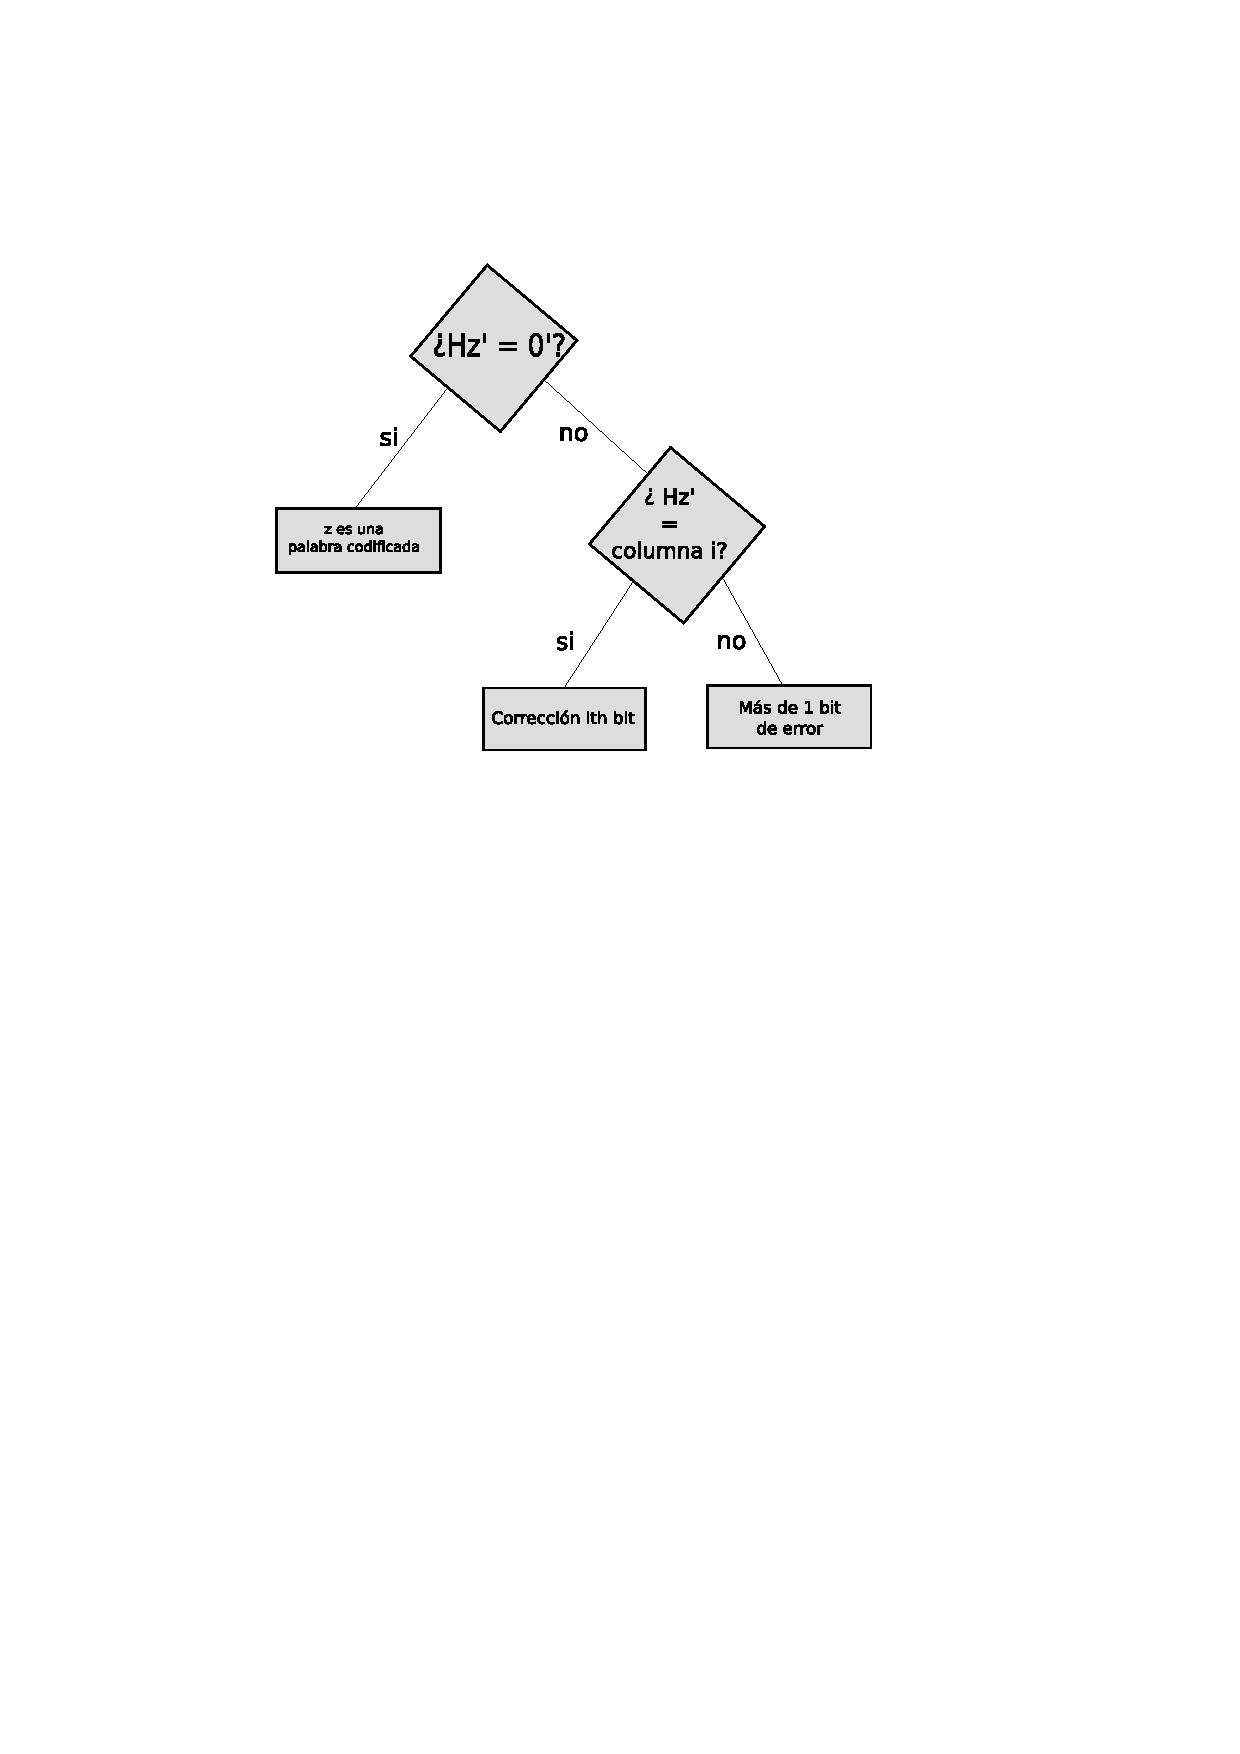
\includegraphics[height=0.5\textheight]{esquemaH.pdf} 
\end{center}
\caption{\footnotesize Procesando palabra recibida $z$ para código matriz de verificación $H$}\label{fig:esquemaH}
\end{figure}

\end{frame} 

%%%%%%%%%%%%%%%%%%%%%%%%%%%%%%%%
%\begin{frame}  \small  
%\begin{itemize} 

%\item Para cada palabra recibida $z$ el Receptor deber calcular $Hz'$. 

%\item Si $Hz'=0$, entonces z es la palabra codificada correcta. 

%\item Si $Hz'$ es igual a la columna $i^{th}$ de $H$, entonces la palabra codificada correcta es obtenida cambiando el $i^{th}$ bit en z. 
%\item En otro caso, al menos dos bit son erróneos. 


%\end{itemize} \end{frame} 

%%%%%%%%%%%%%%%%%%%%%%%%%%%%%%%%
%%%%%%%%%%%%%%%%%%%%%%%%%%%%%%%%
%\begin{frame}  \small \begin{ejercicio} \end{ejercicio} \pause \textit{\underline{Solución}}:\\ \end{frame} 
%%%%%%%%%%%%%%%%%%%%%%%%%%%%%%%%
%%%%%%%%%%%%%%%%%%%%%%%%%%%%%%%%
%EJERCICIO %%%%%%%%%%%%%%%%%%%%%%%%%%%%%%%
%%%%%%%%%%%%%%%%%%%%%%%%%%%%%%%%

%%%%%%%%%%%%%%%%%%%%%%%%%%%%%%%%
%%%%%%%%%%%%%%%%%%%%%%%%%%%%%%%%
\begin{frame}  \small \begin{ejercicio} 
Construya un Código Corrector 1  $C \in \mathbb{F}_2^6$  con $|C| = 8$.

\end{ejercicio} %\pause 
\textit{\underline{Solución}}:\\ 
\vspace{0.3cm}

H es una matriz $m \times n$ con m=n-k.

Del enunciado sabemos que n=6 y k=3, por lo que debemos construir una matriz $3 \times 6$.

\[
        \left( \begin{array}{ccccccc}
                  x_1 & x_2 & x_3 & x_4 & x_5 & x_6  & peso\\
                      1 &   1   &   1  &    1 &   0  &   0    &4\\  
					  1 &   1   &   0  &    0 &   1  &   0	  &3\\ 
					  1 &   0   &   1  &    0 &   0  &   1	  &3
           			\end{array}
    		\right) 	    		
\]

\end{frame} 
%%%%%%%%%%%%%%%%%%%%%%%%%%%%%%%%


%%%%%%%%%%%%%%%%%%%%%%%%%%%%%%%%
%%%%%%%%%%%%%%%%%%%%%%%%%%%%%%%%
%\begin{frame}  \small \begin{ejercicio} \end{ejercicio} \pause \textit{\underline{Solución}}:\\ \end{frame} 
%%%%%%%%%%%%%%%%%%%%%%%%%%%%%%%%


%8.14. Find the smallest values of n and k for which a 1-error correcting code with information rate 0.75 can exist, and explain how to define such a code by means of a check matrix.

%8.15. Write down all the codewords belonging to the linear code with the following check matrix, and find the parameters (n,k,δ) for this code.

%%%%%%%%%%%%%%%%%%%%%%%%%%%%%%%%
%%%%%%%%%%%%%%%%%%%%%%%%%%%%%%%%
\begin{frame}  \small \begin{ejercicio} 

Establezca todas las palabras codificadas que pertenecen a un código lineal con la siguiente matriz de verificación, y encuentra los parámetros $(n,k,\delta)$ para este código.

\[
        \left( \begin{array}{ccccccc}
                      1 &   1   &   0  &    1 &   0  &   0    &1\\  
					  0 &   0   &   0  &    1 &   1  &   0	  &1\\ 
					  1 &   0   &   1  &    1 &   0  &   0	  &1\\
					  0 &   0   &   0  &    0 &   0  &   1	  &1\\
           			\end{array}
    		\right) 	    		
\]
\end{ejercicio}  \end{frame} 
%%%%%%%%%%%%%%%%%%%%%%%%%%%%%%%%

\begin{frame}  \tiny
\textit{\underline{Solución}}:\\

La matriz identidad está formada por las columnas 2,5,3  y 6. Esto significa que $x_2$, $x_5$, $x_3$ y $x_6$ pueden ser determinadas por $x_1$, $x_4$ y $x_7$. Explícitamente podemos determinar estas ecuaciones de la forma:

\begin{center}
$x_2=x_1+x_4+x_7$\\
$x_5= x_4 + x_7$\\
$x_3=x_1 + x_4 + x_7$\\
$x_6 = x_7$\\
\end{center}

Por tanto, tenemos 8 palabras codificadas determinadas por los bits $x_1$, $x_4$ y $x_7$ $(2^3)$.\\

\begin{center}
$x_1= 0$, $x_4= 0$, $x_7=0$ tendremos $x_2=0$, $x_3=0$, $x_5=0$, $x_6=0$ $\mapsto 0000000$\\
$x_1= 0$, $x_4= 0$, $x_7=1$ tendremos $x_2=1$, $x_3=1$, $x_5=1$, $x_6=1$ $\mapsto 0110111$\\
$x_1= 0$, $x_4= 1$, $x_7=0$ tendremos $x_2=1$, $x_3=1$, $x_5=1$, $x_6=0$ $\mapsto 0111100$\\
$x_1= 0$, $x_4= 1$, $x_7=1$ tendremos $x_2=0$, $x_3=0$, $x_5=0$, $x_6=1$ $\mapsto 0001011$\\

$x_1= 1$, $x_4= 0$, $x_7=0$ tendremos $x_2=1$, $x_3=1$, $x_5=0$, $x_6=0$ $\mapsto 1110000$\\
$x_1= 1$, $x_4= 0$, $x_7=1$ tendremos $x_2=0$, $x_3=0$, $x_5=1$, $x_6=1$ $\mapsto 1000111$\\
$x_1= 1$, $x_4= 1$, $x_7=0$ tendremos $x_2=0$, $x_3=0$, $x_5=1$, $x_6=0$ $\mapsto 1001100$\\
$x_1= 1$, $x_4= 1$, $x_7=1$ tendremos $x_2=1$, $x_3=1$, $x_5=0$, $x_6=1$ $\mapsto 1111011$\\
\end{center}

Sabemos n=7, k=3 y $\delta=3$ que es la mínima distancia posible para código corrector 1.

 \end{frame} 
%%%%%%%%%%%%%%%%%%%%%%%%%%%%%%%%

%%%%%%%%%%%%%%%%%%%%%%%%%%%%%%%%
%%%%%%%%%%%%%%%%%%%%%%%%%%%%%%%%
\begin{frame}  \small \begin{ejercicio} 

Una palabra codificada del código definido por la siguiente matriz ha sido enviada, y la palabra 111010 ha sido recibida.

\[
        \left( \begin{array}{cccccc}
                      1 &   1   &   1  &    1 &   0  &   0  \\  
					  1 &   1   &   0  &    0 &   1  &   0	\\ 
					  1 &   0   &   1  &    0 &   0  &   1	\\
           			\end{array}
    		\right) 	    		
\]

¿Cual es la palabra codificada, asumiendo que solamente un error ha ocurrido?

\end{ejercicio} %\pause 
\textit{\underline{Solución}}:\\ 
\vspace{0.3cm}

Dada z'=[111010]', encontramos Hz'=[110]', que coincide con la 2 columna de H, por lo que el error ha sido en el 2 bit.

La palabra correcta es c=101010 y ahora Hc=0'.

 \end{frame} 
%%%%%%%%%%%%%%%%%%%%%%%%%%%%%%%%


%%%%%%%%%%%%%%%%%%%%%%%%%%%%%%%%
%%%%%%%%%%%%%%%%%%%%%%%%%%%%%%%%
\begin{frame}  \small \begin{ejercicio} 

En el ejercicio anterior, ¿Cuantas palabras no pueden ser corregidas, bajo la suposición que al menos un error ha ocurrido?

\end{ejercicio} %\pause 
\textit{\underline{Solución}}:\\ 
\vspace{0.3cm}

\begin{itemize}
\item n= 6, por lo que tenemos $2^6=64$ palabras y $2^3=8$ palabras codificadas. 
\item Cada $N_1(c)$ contiene 6+1 elementos. 
\item Por tanto 8 x 7 palabras pueden ser corregidas.
\item Por lo que 64 - 56= 8 palabras no pueden ser corregidas.

\end{itemize}





\end{frame} 
%%%%%%%%%%%%%%%%%%%%%%%%%%%%%%%%





%8.16. In Exercise 8.2 we showed that it is impossible to encode 128 different messages in such a way that one error is corrected, using binary words of length 10. Explain how to construct a linear code satisfying the conditions, using words of length 11.

%8.17. A codeword from the code defined by the following check matrix is sent, and the word 111010 is received.
%111100 110010. 101001 What was the intended codeword, assuming that only one error has been made?

%8.18. In the preceding exercise, how many received words cannot be cor- rected on the assumption that at most one error has been made?


%%%%%%%%%%%%%%%%%%%%%%%%%%%%%%%%
%%%%%%%%%%%%%%%%%%%%%%%%%%%%%%%%
%SECCION %%%%%%%%%%%%%%%%%%%%%%%%%%%%%%%
%%%%%%%%%%%%%%%%%%%%%%%%%%%%%%%%
\section{El problema de la decodificación}

\begin{frame}   \footnotesize
{
\setbeamercolor{block title}{bg=blue!60!black, fg=white}
\setbeamercolor{block body}{bg=blue!10, fg=black}
\begin{block}{Sección 5}
El problema de la decodificación
\end{block}
}
\end{frame} 
%%%%%%%%%%%%%%%%%%%%%%%%%%%%%%%%
\begin{frame}  \frametitle{El problema de la decodificación}\footnotesize
\begin{itemize} 

\item  De forma genérica, no hay una forma fácil de implementar \textbf{la regla de decisión MD}. Podemos utilizar el método por fuerza bruta mediante una lista de todas las palabras codificadas, pero no es un método eficiente.

\item Generalmente el problema de decodificación puede ser simplificado utilizando una técnica conocida como \textbf{decodificación por síndrome}.

\end{itemize} 

\begin{definicion}[Síndrome]\footnotesize

\begin{itemize}
\item Sea \textbf{C el código lineal definido por una matriz de verificación H}. 

\item Para cualquier palabra $z \in \mathbb{F}_2^n$ el \textbf{síndrome} de $z$ es $s$, donde $Hz'=s'$.

\item Si $z$ es una \textbf{palabra codificada} entonces el \textbf{síndrome} de $z$ es la palabra \textbf{cero} $(s'=0)$. 

\item Si $z$ es el resultado de realizar \textbf{un simple error}, en el $i^{th}$ de una palabra codificada, entonces el \textbf{síndrome} es la palabra en la $i^{th}$ columna de $H$.

\end{itemize}

\end{definicion}

\begin{lema}
Dos palabras $y, z \in \mathbb{F}_2^n$ tiene el mismo síndrome con respecto a C sii $y= z+c$, para algún $c\in C$.
\end{lema}



\end{frame} 

%%%%%%%%%%%%%%%%%%%%%%%%%%%%%%%%

\begin{frame}  \small  

\begin{itemize}
\item El conjunto de $y \in \mathbb{F}_2^n$ tal que y=z+c para algún $c \in C$ es conocido como la \textbf{clase de equivalencia de z} con respecto a C y es denotado como \textbf{z+C}. 


\item La Teoría elemental de Grupo define que dos \textbf{clases de equivalencia} son \textbf{disjuntos} o \textbf{idénticas} (no pueden parcialmente coincidir), por lo que \textbf{distintas clases de equivalencia forman una partición de} $\mathbb{F}_2^n$.


\end{itemize}


\end{frame} 


%%%%%%%%%%%%%%%%%%%%%%%%%%%%%%%%
\begin{frame}  \small  

\begin{ejemplo}\label{ej:Coset}
Enumera las clases de equivalencia del código $C \subseteq \mathbb{F}_2^4$ definida por la matriz de verificación.

\[
   H=      \left( \begin{array}{cccc}
                  1 & 0 & 1 & 0\\
                  1 & 1 & 0 & 1 	  
           			\end{array}
    		\right) 	    		
\]
\end{ejemplo}

\

   

\end{frame} 
%%%%%%%%%%%%%%%%%%%%%%%%%%%%%%%%
\begin{frame}  \footnotesize


\textit{\underline{Solución}}:\\
\vspace{0.2cm}

En el ejemplo \ref{ej:CodeMatrizV} mostraremos que C contiene cuatro palabras codificadas 0000, 0101, 1011, 1110.\\
\vspace*{4pt}
Ya que $|C| = 4$ y $|F_2^4| = 2^4 = 16$, hay 16/4 = 4 clases de equivalencias distintas.\\
\vspace*{4pt}
La primera clase de equivalencia la construimos con $z_1$=0000, siendo la propia C, 0000+C\\
\vspace*{4pt}
Las distintas \textbf{clases de equivalencias}, $z_i$+C, escogiendo cualquier z que \textbf{no} este en las anteriores clases de equivalencias, por ejemplo $z_2$=1000, $z_3$=0100 y $z_4$=0010. De esta forma, tenemos cuatro clases de equivalencias distintas:
\vspace*{4pt}
\tiny
\[
  \begin{array}{cccc}
          \textcolor{red}{\textbf{0000+C}} & \textcolor{red}{\textbf{1000+C}}  & \textcolor{red}{\textbf{0100+C}} & \textcolor{red}{\textbf{0010+C}} \\
                   &  &  & \\	
                    \textcolor{blue}{\textbf{0000}} & \textcolor{blue}{\textbf{1000}} & \textcolor{blue}{\textbf{0100}}	 & \textcolor{blue}{\textbf{0010}}\\ 
				    0101 & 1101 & \textcolor{olive}{\textbf{0010}}  & 0111\\
					1011 & 0011 & 1111 & 1001\\
				    1110 & 0110 & 1010 &	1100\\
           			\end{array}
\]
   

\end{frame} 


%%%%%%%%%%%%%%%%%%%%%%%%%%%%%%%%
\begin{frame}  \footnotesize
\begin{itemize} 

\item Si el código tiene longitud de palabra n y dimensión k, el \textbf{número de clases de equivalencias} es $2^n / 2^k = 2^{n-k} =2^m$, donde m es el número de filas de H. 

\item \textcolor{red}{\textbf{Síndrome}} es una palabra de longitud \textbf{m} ($ s'= H z'$), y diferentes clases de equivalencias tienen diferentes síndromes, todas las posibles palabras en $\mathbb{F}_2^m$ se dan como síndromes.

\item  Es conveniente ordenarlos en un orden definitivo, como por ejemplo el orden de diccionario. 

\end{itemize} 
\begin{definicion}[Líder Clase de Equivalencia, Tabla  de asignación de síndromes]

Un \textbf{líder de la clase de equivalencia} es una palabra de menor peso en su clase de equivalencia, si existe varias posibilidades, escogeremos una de ellas.\\
\vspace*{10pt}
\textbf{Tabla de asignación de síndromes}  es una lista ordenada de pares (s,f) de tal forma que, para cada síndrome s, f es el líder de la clase de equivalencia para la clase de equivalencia que tiene el síndrome s.
\end{definicion}

\end{frame} 

%%%%%%%%%%%%%%%%%%%%%%%%%%%%%%%%
\begin{frame}  \small  
\begin{enumerate} 



\item  Lista de \textbf{clases de equivalencia} del ejemplo \ref{ej:Coset}, escogemos el elemento que tiene menor peso, y en caso de empate cualquiera de los dos y lo establecemos como líder. 

\item Calculamos los \textbf{síndromes} con los líderes de la clase de equivalencia:


\[
   H=      \left( \begin{array}{cccc}
                  1 & 0 & 1 & 0\\
                  1 & 1 & 0 & 1 	  
           			\end{array}
    		\right) 	    		
\]
\begin{center}
$\mathbf{s_0} = H \;\mathbf{z_0} = H \;$ 0000 =  00 \hspace{0.2cm}
$\mathbf{s_1} = H \;\mathbf{z_1} = H \;$ \textcolor{red}{1000} =  \textcolor{red}{11}\\
$\mathbf{s_2} = H \;\mathbf{z_2} = H \;$ \textcolor{blue}{0100} =  \textcolor{blue}{01} \hspace{0.2cm}
$\mathbf{s_3} = H \;\mathbf{z_3} = H \;$ \textcolor{olive}{0010} =  \textcolor{olive}{10}

\end{center}

\item Ordenamos los síndromes en un \textbf{orden de diccionario}, la \textbf{tabla de asignación} de síndrome quedaría de la siguiente forma:


\[
  \begin{array}{lcccc}
                   sindrome & 00 & \textcolor{blue}{01} & \textcolor{olive}{10} & \textcolor{red}{11}\\ 
				   lider\, clase\, eq. & 0000 & \textcolor{blue}{0100} & \textcolor{olive}{0010} & \textcolor{red}{1000}
	\end{array}
\]
\end{enumerate} \end{frame} 


%%%%%%%%%%%%%%%%%%%%%%%%%%%%%%%%
\begin{frame}  \small  

El \textcolor{red}{\textbf{método de decodificación del síndrome}} está basado en el supuesto que 
\begin{enumerate}
    \item el Receptor conoce que la \textbf{matriz de verificación} $H$ para un código C y
 \item  tiene una copia de la \textbf{tabla de asignación}.
\end{enumerate}

\vspace*{3pt}

En ese caso, la siguiente \textbf{regla de decisión} $\sigma:\mathbb{F}_2^n \rightarrow C$ puede ser aplicada:

\begin{enumerate}
\item Para una palabra recibida z, calcular el \textbf{síndrome} s, utilizando la ecuación $s'=Hz'$
\item Establecer el \textbf{líder de la clase de equivalencia} $f$ correspondiente a $s$
\item Calcular $\sigma(z)= z+f$
\end{enumerate}


\begin{teorema}

Con la notación utilizada anteriormente:
\begin{enumerate}
\item $\sigma(z)= z+f$ es una palabra codificada
\item No existe palabra codificada $c\in C$ tal que $d(z,c) < d(z,z + f).$
\end{enumerate}

\end{teorema}

\end{frame} 



%%%%%%%%%%%%%%%%%%%%%%%%%%%%%%%%
\begin{frame}  \small  
\begin{ejemplo}

La matriz de verificación 

\[
   H=      \left( \begin{array}{ccccc}
                  1 & 0 & 1 & 0 & 0\\
                  1 & 1 & 0 & 1 & 0\\	  
                  0 & 1 & 0 & 0 & 1
           			\end{array}
    		\right) 	    		
\]

define el código $C = \{00000, 01011, 10110, 11101\}$.\\
\vspace*{13pt}
Construye una \textbf{tabla de asignación de síndromes} para C y utilízalo para determinar  $\sigma (10111)$.
\end{ejemplo}

\end{frame} 


%%%%%%%%%%%%%%%%%%%%%%%%%%%%%%%%
\begin{frame}  \footnotesize  

\textit{\underline{Solución}}:\\
\vspace{0.3cm}

\vspace*{3pt}
La primera clase de equivalencia es 00000 + $C = \{00000, 01011, 10110, 11101\}$. \\
\vspace*{3pt}

\tiny
\[
  \begin{array}{c}
          \textcolor{red}{\textbf{00000+C}} \\
                    \textcolor{blue}{00000} \\ 
				    01011 \\
					10110 \\
				    11101 \\
           			\end{array}
\]
\footnotesize
Por ejemplo 00001 no está en la clase de equivalencia, por lo que la próxima clase de equivalencia es 00001 + C. Continuando de esta forma podemos obtener \textbf{ocho} clases de equivalencia

\begin{center}
\textbf{00000}+C \textbf{00001}+C \textbf{00010}+C \textbf{00100}+C\\
\textbf{01000}+C \textbf{10000}+C \textbf{00101}+C \textbf{00111}+C\\
\tiny
\[
  \begin{array}{lcccccccc}
\textcolor{red}{00000+C} &   \textcolor{red}{00001+C} &   \textcolor{red}{00010+C} &   \textcolor{red}{00100+C} 
&   \textcolor{red}{01000+C} &   \textcolor{red}{10000+C} &   \textcolor{red}{00101+C} &   \textcolor{red}{00111+C}
\\
\textbf{00000} & \textbf{00001} &	\textbf{00010} &	\textbf{00100} 	& \textbf{01000} 	&	\textbf{10000} &	\textbf{00101} &   00111\\
01011	& 01010	& 01001	 & 01111	&00011	    &11011 	    &	01110       & \textbf{01100}\\		
10110	& 10111	& 10100	 & 10010	&11110		&00110 		&	10011  		&  10001\\
11101	& 11100	& 11111	 & 11001	&10101		&01101 		&	11000 		&  11010
\end{array}  		
\]
\footnotesize

\end{center}

\end{frame} 

%%%%%%%%%%%%%%%%%%%%%%%%%%%%%%%%
\begin{frame}  \footnotesize  

Por ejemplo,  la clase de equivalencia 00111 + C contiene las palabras 00111, 01100 10001, y 11010. Por lo que el líder de la clase de equivalencia puede ser  \textbf{01100} o \textbf{10001}. Supongamos que escogemos \textbf{01100} como el líder de esta clase de equivalencia, y realizamos elecciones similares para otras clases de equivalencia. \\

\vspace*{13pt}

Para cada \textbf{líder de las clases de equivalencia} $f$, el síndrome $s$  para todas las palabras de esa clase de equivalencia es dado por $s' = H' f$. Ahora debemos crear \textbf{la tabla de asignación de síndromes} para C según las elecciones realizadas.

\[
    \begin{array}{cccccccc}
               000	& 001	& 010	& 011&	100	&101	&110	&111\\
00000 & 00001& 00010 & 01000 & 00100 & 00101 & 10000& 01100
           			\end{array}  		
\]

\vspace*{0.3cm}

La palabra recibida es z = 10111. \\

\vspace*{0.3cm}

Calculamos $Hz' = 001'$ el correspondiente líder de la clase de equivalencia es f = \textbf{00001} y la decisión del Receptor sera que $\sigma(z) = z + f = $ \textbf{10110}.


\end{frame} 

%%%%%%%%%%%%%%%%%%%%%%%%%%%%%%%%
\begin{frame}  \small  
\begin{itemize} 

\item  El método de decodificación por síndrome, \textcolor{red}{\textbf{no siempre mejora el método de fuerza bruta} para implementar la \textbf{regla MD}}. 

    \begin{itemize} 
        \item En el método de \textbf{fuerza bruta}, si la palabra recibida $z$  es comparada con cada palabra codificada para encontrar cual es la más cercana, entonces, para un código lineal de dimensión $k$, necesitaremos $2^k$ \textbf{comparaciones}. 
        \vspace{0.3cm}
        \item Con la decodificación por síndrome el \textbf{Receptor} debe tener una \textbf{copia de la tabla de asignación}, que contiene $2^{n-k}$ entradas, que puede ser considerado como un número grande.
    \end{itemize}


\item  Afortunadamente, cuando los códigos son construidos utilizando \textbf{métodos algebraicos} hay mejores formas de implementar la \textbf{regla MD}.



\end{itemize} \end{frame} 

%%%%%%%%%%%%%%%%%%%%%%%%%%%%%%%%
%%%%%%%%%%%%%%%%%%%%%%%%%%%%%%%%
%\begin{frame}  \small \begin{ejercicio} \end{ejercicio} \pause \textit{\underline{Solución}}:\\ \end{frame} 
%%%%%%%%%%%%%%%%%%%%%%%%%%%%%%%%
%%%%%%%%%%%%%%%%%%%%%%%%%%%%%%%%
%EJERCICIO %%%%%%%%%%%%%%%%%%%%%%%%%%%%%%%
%%%%%%%%%%%%%%%%%%%%%%%%%%%%%%%%

%%%%%%%%%%%%%%%%%%%%%%%%%%%%%%%%
%%%%%%%%%%%%%%%%%%%%%%%%%%%%%%%%
\begin{frame}  \small \begin{ejercicio} 

Construir una tabla de asignación de síndromes para el código definido por la matriz de verificación

\[
      \left( \begin{array}{ccccc}
                  1 & 0 & 1 & 0 & 0\\
                  0 & 1 & 0 & 1 & 0\\	  
                  1 & 1 & 0 & 0 & 1
           			\end{array}
    		\right) 	    		
\]

\vspace{0.3cm}
Utilizar la tabla para determinar las palabras codificadas correspondientes a las siguientes palabras:
11111, 11010, 01101, 01110.

\end{ejercicio} 
\end{frame} 
%%%%%%%%%%%%%%%%%%%%%%%%%%%%%%%%

\begin{frame}  \footnotesize

 \textit{\underline{Solución}}:\\ 
\vspace{0.3cm}

$x_3=x_1$\\
$x_4=x_2$\\
$x_5=x_1+x_2$\\

\[
  \begin{array}{lcccccccc}
\textbf{00000}		& \textbf{00001}	& 	\textbf{00010}	& 	00011			& 		\textbf{00100}		& 00101		& 			00110		& 		00111\\
01011		& 01010					& 01001			& 		\textbf{01000}	& 	01111			& 		01110	& 				01101	& 		\textbf{01100}\\
10101		& 			10100			& 		10111		& 			10110			& 		10001		& 			\textbf{10000}	& 	10011	& 				10010\\
11110      & 			11111			& 		11100		& 			11101			& 		11010		& 			11011			& 		\textbf{11000}	& 	11001\\
	\end{array}
\]

\[
  \begin{array}{lcccccccc}
                   sindrome 				& 000 & 001	 	  & 010 	& 011		& 100     & 101	 	  & 110 	& 111\\ 
				   lider\, clase\, eq. & 0000 & 00001 & 00010 & 01000   & 00100 & 10000  & 11000 & 01100
	\end{array}
\]


\begin{center}
11111, s =H z= 001, f = 00001, $\sigma (z)$ = 11111 + 00001=11110\\
11010, s =H z= 100, f = 00100, $\sigma (z)$ = 11010 + 00100=11110\\
01101, s =H z= 110, f = 11000, $\sigma (z)$ = 01101 + 11000=10101\\
01110, s =H z= 101, f = 10000, $\sigma (z)$ = 01110 + 10000=11110\\
\end{center}

\end{frame} 
%%%%%%%%%%%%%%%%%%%%%%%%%%%%%%%%



%\begin{frame}  \footnotesize

% \textit{\underline{Solución}}:\\ 
%\vspace{0.3cm}
%\[
%  \begin{array}{lcc}
%                   	& 01101 & 00111\\ 
%     	 00000 &  3 		&	  3	\\
%     	 01011 &  2		&	 2	\\
%     	 10101 &  2		&	2	\\
%     	 11110 &  3		&	3	\\
%	\end{array}
%\]


%\end{frame} 

%8.20. Suppose the Sender uses the code C = {00000, 01011, 10110, 11101}
%and the Receiver uses the syndrome look-up table for C given in Ex- ample 8.18. Given that the probability of a bit-error in transmission is e, estimate M0, the probability of a mistake when the codeword 00000 is sent.

%8.21. Denote by hi the column 4-vector corresponding to the binary rep- resentation of the integer i (1 ≤ i ≤ 15). For example, h9 = [1001]′. Let H be the 8 × 15 binary matrix with the first four rows
%h1 h2 h3 h4 h5 h6 h7 h8 h9 h10 h11 h12 h13 h14 h15, and the last four rows
%h5 h3 h1 h1 h8 h15 h1 h15 h8 h5 h5 h8 h3 h15 h3.
%H is the check matrix for a code C ⊆ F215. A codeword c ∈ C is transmitted and the received word is
%z = 100100100100000.
%Calculate the syndrome of z. How do we know that z is not a code- word, and that more than one bit-error has been made? Assuming that exactly two bit-errors have been made, which two bits should be corrected? [The general construction of which this is an example will be discussed in the next chapter.]

%%%%%%%%%%%%%%%%%%%%%%%%%%%%%%%%
%\begin{frame}  \small  
%\end{frame} 


%%%%%%%%%%%%%%%%%%%%%%%%%%%%%%%%
%\begin{frame}  \small  
%\begin{itemize} \item  \item \item \item 
%\end{itemize} \end{frame} 

%%%%%%%%%%%%%%%%%%%%%%%%%%%%%%%%
%\begin{frame}  \small \begin{ejercicio} \end{ejercicio}\end{frame} 



\begin{frame} %\frametitle{Preguntas}

%\begin{center}
%¡Gracias por su atención!\\
%\end{center}
\vspace*{2cm}

\begin{center}
\textbf{José A. Montenegro Montes} \\

\textit{Dpto. Lenguajes y Ciencias de la Computación}\\
\textit{ETSI  Informática. Universidad de Málaga}\\
\textbf{jmmontes@uma.es}\\
%\href{https://twitter.com//monteDocencia}{
%
\includegraphics[height=0.05\textheight]{twitter.jpg}}
\end{center}

\vspace*{1,5cm}


\includegraphics[height=0.15\textheight]{logoUma.jpg} \hspace*{3.6cm}

\includegraphics[height=0.15\textheight]{logoInf.jpg}   \hspace*{3.7cm}

\includegraphics[height=0.15\textheight]{logoLcc.jpg}  




\end{frame} 

\end{document} 